\chapter{Operational Amplifier }
\section{Introduction}
An operational amplifier is a direct-coupled high-gain amplifier usually consisting of one or more differential amplifiers.\\ The operational amplifier is a versatile device that can be used to amplify dc as well as ac input signals and was originally designed for performing mathematical operations such as addition, subtraction, multiplication, and integration. Thus the name operational amplifier stems from its original use for these mathematical operations and is abbreviated to $o p-a m p$. With the addition of suitable external feedback components, the modern day op-amp can be used for a variety of applications, such as ac and dc signal amplification, active filters, oscillators, comparators, regulators, and others.

\begin{figure}[H]
	\centering
	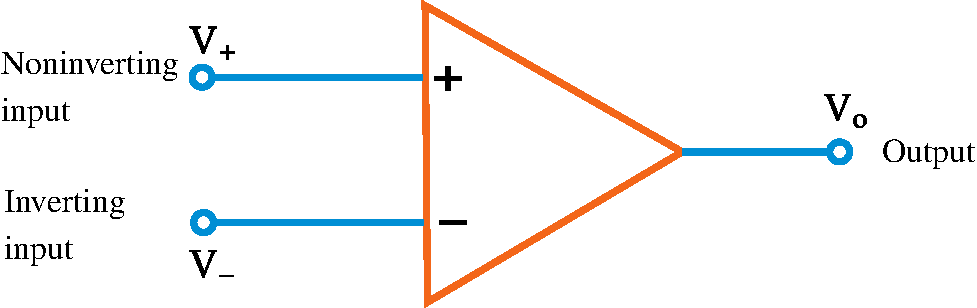
\includegraphics[height=2.2cm,width=7cm]{Opamp schematic}
	\caption{Schematic diagram of an an op-amp}
	\label{Opamp schematic}
\end{figure}
$\left. \right. $\\
 A  schematic diagram of an an op-amp is shown in the figure.\ref{Opamp schematic}. \\
  For  simplicity, power supply and other pin connections are omitted. Since the input differential amplifier stage of the op-amp is designed to be operated in the differential mode, the differential inputs are designated by the $(+)$ and $(-)$ notations. The $(+)$ input is the noninverting input. An ac signal (or dc voltage) applied to this input produces an in-phase (or same polarity) signal at the output. On the other hand, the $(-)$ input is the inverting input because an ac signal (or dc voltage) applied to this input produces an $180^{\circ}$ out-of-phase (or opposite polarity) signal at the output.
   In Figure,
   $$
   \begin{aligned}
   \mathrm{V_{+}}&=\text { Voltage at the noninverting input (volts) } \\
   \mathrm{V_{-}}&=\text { Voltage at the inverting input (volts) } \\
   \mathrm{V_{o}}&=\text { Output voltage (volts) }
   \end{aligned}
   $$
   All these voltages are measured with respect to ground.

  \section{Op-Amp characterestics}
  \subsection{Input offset voltage} 
  
   \begin{figure}[H]
   	\centering
   	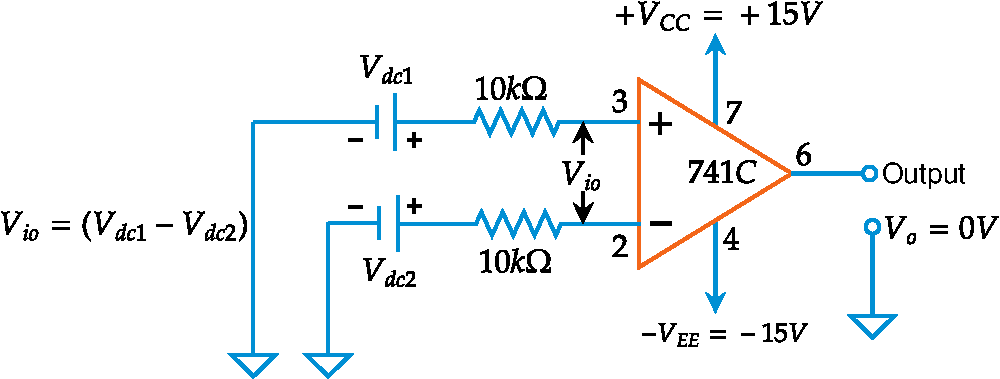
\includegraphics[height=4.5cm,width=11cm]{Input offset voltage}
   	\caption{Defining input offset voltage}
   	\label{Input offset voltage}
   \end{figure}
   \par Input offset voltage is the voltage that must be applied between the two input terminals of an op-amp to null the output, as shown in Figure.\ref{Input offset voltage}. In the figure $V_{\mathrm{dc} 1}$ and $V_{\mathrm{dc} 2}$ are dc voltages and $R_{S}$ represents the source resistance. We denote input offset voltage by $V_{i o}$. This voltage $V_{i o}$ could be positive or negative; therefore, its absolute value is listed on the data sheet. For a $741 \mathrm{C}$ the maximum value of $V_{i o}$ is $6 \mathrm{mV} \mathrm{dc}$. The smaller the value of $V_{i o}$, the better the input terminals are matched. For instance, the $714 \mathrm{C}$ precision op-amp has $V_{i o}=150 \mu \mathrm{V}$ maximum.
   \subsection{Input offset current}
   \begin{figure}[H]
   	\centering
   	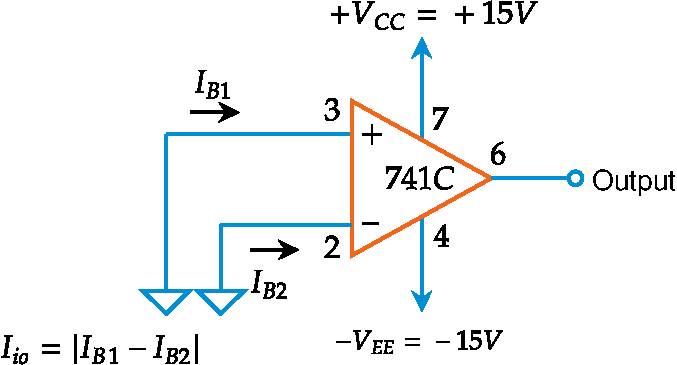
\includegraphics[height=4.5cm,width=8cm]{Input offset current}
   	\caption{Defining input offset current}
   	\label{Input offset current}
   \end{figure}
    The algebraic difference between the currents into the inverting and noninverting terminals is referred to as input offset current, $I_{i o}$. In the form of an equation,
   $$
   I_{i o}=\left|I_{B 1}-I_{B 2}\right|
   $$
   where $I_{B 1}$ is the current into the noninverting input and $I_{B 2}$ is the current into the inverting input.
   \subsection{Input bias current}
   Input bias current, $I_{B}$, is the average of the currents that flow into the inverting and noninverting input terminals of the op-amp. In equation form,
   $$
   I_{B}=\frac{I_{B 1}+I_{B 2}}{2}
   $$
   $I_{B}=500 \mathrm{nA}$ maximum for the $741 \mathrm{C}$, whereas $I_{B}$ for the precision $714 \mathrm{C}$ is $\pm 7 \mathrm{nA} .$ \\
   Note that the two input currents $I_{B 1}$ and $I_{B 2}$ are actually the base currents of the first differential amplifier stage.
   \subsection{Differential input resistance}
   Differential input resistance, $R_{i}$, (often referred to as input resistance) is the equivalent resistance that can be measured at either the inverting or noninverting input terminal with the other terminal connected to oround. For the $741 \mathrm{C}$ the input resistance is a relatively high $2 \mathrm{M} \Omega$.
   \subsection{Common Mode Rejection Ratio (CMRR)}
  \textbf{The common-mode rejection ratio (CMRR) }is defined in several essentially equivalent ways by various manufacturers. Generally, it can be defined as the ratio of the differential voltage gain $A_{d}$ to the common-mode voltage gain $A_{\mathrm{cm}} $ that is,
   \begin{equation}
   \mathrm{CMRR}=\frac{A_{d}}{A_{\mathrm{cm}}}
   \end{equation}
  
   The differential voltage gain $A_{d}$ is the same as the large-signal voltage gain $A$, which is specified on the data sheets; however, the common-mode voltage gain can be determined from  using the equation,
   \begin{equation}
  \mathrm{A}_{\mathrm{cm}}=\frac{V_\mathrm{ocm}}{V_{\mathrm{cm}}}
   \end{equation}
   $$
   \begin{aligned}
   \text{Where ,} V_\mathrm{ocm}&= \text{output common-mode voltage}\\
   V_{\mathrm{cm}}&=\text { input common-mode voltage } \\
   A_{\mathrm{cm}}&=\text { common-mode voltage gain }
   \end{aligned}
   $$
   Generally the $A_{\mathrm{cm}}$ is very small and $A_{d}=A$ is very large, therefore, the $\mathrm{CMK}$ is very large. Being a large value, CMRR is most often expressed in decibels (dB). For the $741 \mathrm{C}$, CMRR is $90 \mathrm{~dB}$ typically.
   \begin{note}
   	  \textbf{Common mode voltage:} When the same voltage is applied to both input terminals, the voltage is called a common-mode voltage, $V_{\mathrm{cm}}$, and the op-amp is said to be operating in the common-mode configuration.
   \end{note}
   \subsection{Output resistance}
   Output resistance, $R_{o}$, is the equivalent resistance that can be measured between the output terminal of the op-amp and the ground (or common point). It is $75 \Omega$ for the $741 \mathrm{C}$ op-amp.
   \subsection{Slew rate}
   Slew rate (SR) is defined as the maximum rate of change of output voltage per unit of time and is expressed in volts per microseconds. In equation form,
   $$
   \mathrm{SR}=\left.\frac{d V_{o}}{\mathrm{dt}}\right|_\mathrm{max} \mathrm{V} / \mu \mathrm{s}
   $$
   Slew rate indicates how rapidly the output of an op-amp can change in response to changes in the input frequency. The slew rate changes with change in voltage gain and is normally specified at unity $(+1)$ gain. The slew rate of an op-amp is fixed; therefore, if the slope requirements of the output signal are greater than the slew rate, then distortion occurs. Thus slew rate is one of the important factors in selecting the op-amp for ac applications, particularly at relatively high frequencies.\\
    One of the drawbacks of the $ 741 \mathrm{C}$ is its low slew rate $(0.5 \mathrm{~V} / \mu \mathrm{s})$ 
   \section{The ideal Op-Amp} 
   An ideal op-amp would exhibit the following electrical characteristics,
   \begin{enumerate}
   	\item  Infinite voltage gain $A$.
   	\item Infinite input resistance $R_{i}$ so that almost any signal source can drive it and there is no loading of the preceding stage.
   	\item Zero output resistance $R_{o}$ so that the output can drive an infinite number of other devices.
   	\item Zero output voltage when input voltage is zero.
   	\item Infinite bandwidth so that any frequency signal from 0 to $\infty \mathrm{Hz}$ can be amplified without attenuation.
   	\item Infinite common-mode rejection ratio so that the output common-mode noise voltage is zero.
   	\item Infinite slew rate so that output voltage changes occur simultaneously with input voltage changes.
   \end{enumerate}
   There are practical op-amps that can be made to approximate some of these characteristics using a negative feedback arrangement.
   \newpage
   \begin{abox}
   Practice Set- 1
   \end{abox}
\begin{enumerate}
	\item A time varying signal $V_{i n}$ is fed to an op-amp circuit with output signal $V_{o}$ as shown in the figure below.\\
	\begin{figure}[H]
		\centering
		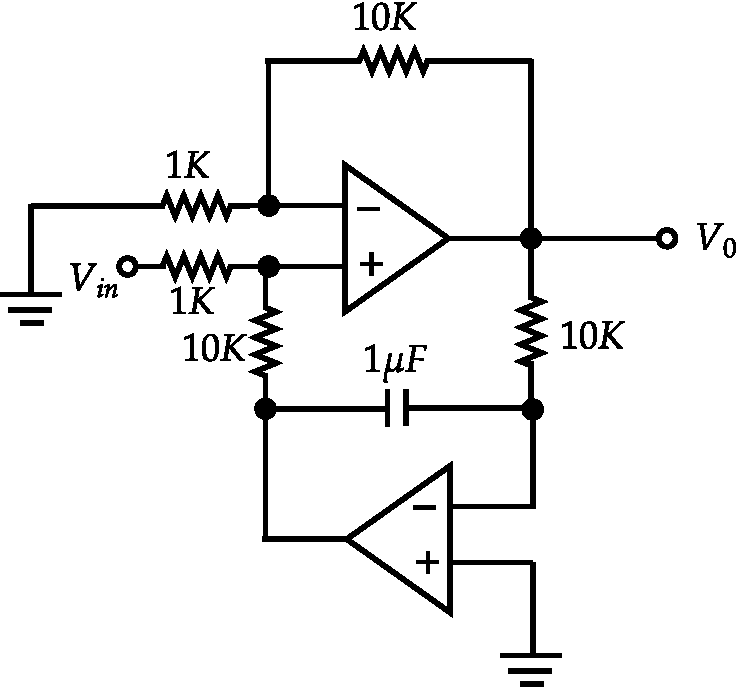
\includegraphics[height=6cm,width=6.5cm]{diagram-20211018(1)-crop}
	\end{figure}
	The circuit implements a
	{\exyear{NET/JRF(JUNE-2011)}}
\begin{tasks}(1)
\task[\textbf{A.}] High pass filter with cutoff frequency $16 \mathrm{~Hz}$
\task[\textbf{B.}] High pass filter with cutoff frequency $100 \mathrm{~Hz}$
\task[\textbf{C.}] Low pass filter with cutoff frequency $16 \mathrm{~Hz}$
\task[\textbf{D.}] Low pass filter with cutoff frequency $100 \mathrm{~Hz}$
\end{tasks}
	\item In the operational amplifier circuit below, the voltage at point $A$ is
{	\exyear{NET/JRF(DEC-2011)}}
\begin{figure}[H]
\centering
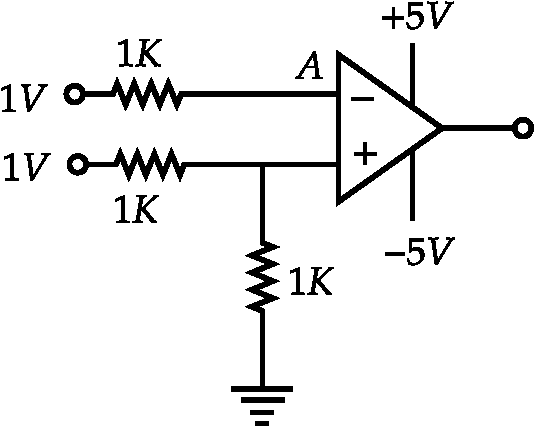
\includegraphics[height=4cm,width=5.5cm]{diagram-20211018(2)-crop}
\end{figure}
\begin{tasks}(4)
\task[\textbf{A.}] $1.0 \mathrm{~V}$
\task[\textbf{B.}] $0.5 \mathrm{~V}$
\task[\textbf{C.}] $0 \mathrm{~V}$
\task[\textbf{D.}] $-5.0 V$
\end{tasks}
	\item In the op-amp circuit shown in the figure below, the input voltage is $1 \mathrm{~V}$. The value of the output $\mathrm{V}_{0}$ is
	{\exyear{NET/JRF(JUNE-2012)}}
\begin{figure}[H]
\centering
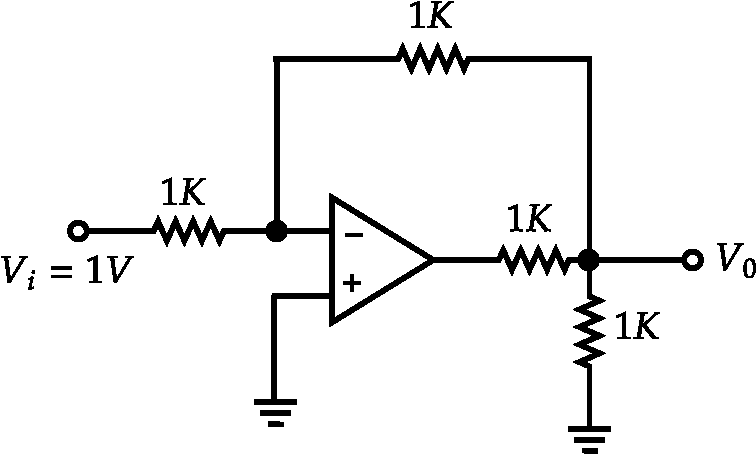
\includegraphics[height=3.5cm,width=6cm]{e-08}
\end{figure}
\begin{tasks}(4)
\task[\textbf{A.}] $-0.33 \mathrm{~V}$
\task[\textbf{B.}] $-0.50 \mathrm{~V}$
\task[\textbf{C.}] $-1.00 \mathrm{~V}$
\task[\textbf{D.}] $-0.25 \mathrm{~V}$
\end{tasks}
	\item In the op-amp circuit shown in the figure, $V_{i}$ is a sinusoidal input signal of frequency 10 $\mathrm{Hz}$ and $V_{0}$ is the output signal. The magnitude of the gain and the phase shift, respectively, close to the values
{	\exyear{NET/JRF(DEC-2012)}}
\begin{tasks}(1)
	\task[\textbf{A.}] $5 \sqrt{2}$ and $\pi / 2$
	\task[\textbf{B.}] $5 \sqrt{2}$ and $-\pi / 2$
	\task[\textbf{C.}] 10 and zero
	\task[\textbf{D.}] 10 and $\pi$
\end{tasks}
\begin{minipage}{0.45\textwidth}
\begin{figure}[H]
	\centering
	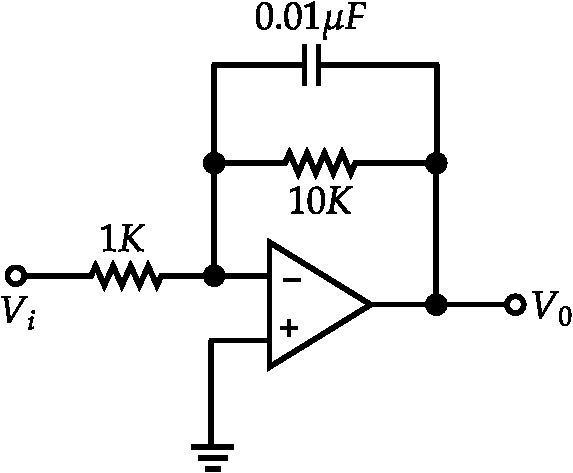
\includegraphics[height=4cm,width=5cm]{e-13}
\end{figure}
\end{minipage}
	\item Consider the op-amp circuit shown in the figure.
	If the input is a sinusoidal wave $V_{i}=5 \sin (1000 t)$, then the amplitude of the output $V_{0}$ is
{	\exyear{NET/JRF(DEC-2013)}}
\begin{figure}[H]
\centering
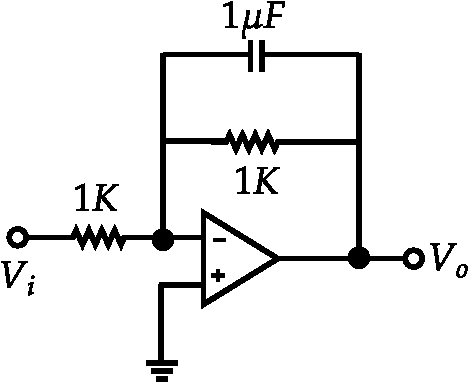
\includegraphics[height=3.5cm,width=4.5cm]{e-21}
\end{figure}
\begin{tasks}(4)
\task[\textbf{A.}] $\frac{5}{2}$
\task[\textbf{B.}]  5
\task[\textbf{C.}] $\frac{5 \sqrt{2}}{2}$
\task[\textbf{D.}] $5 \sqrt{2}$
\end{tasks}
	\item The inner shield of a triaxial conductor is driven by an (ideal) op-amp follower circuit as shown. The effective capacitance between the signal-carrying conductor and ground is
{	\exyear{NET/JRF(JUNE-2014)}}
\begin{figure}[H]
\centering
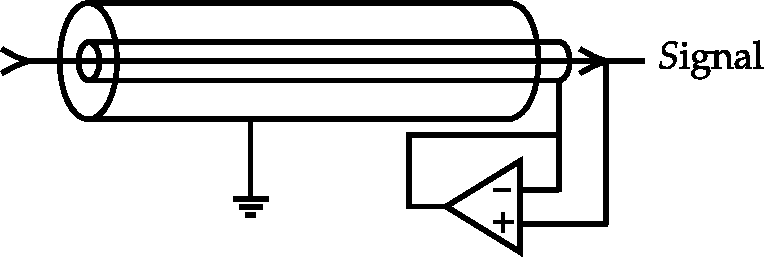
\includegraphics[height=2.5cm,width=7cm]{e-26}
\end{figure}
\begin{tasks}(4)
\task[\textbf{A.}]  Unaffected
\task[\textbf{B.}] Doubled
\task[\textbf{C.}] Halved
\task[\textbf{D.}] Made zero
\end{tasks}
	\item Consider the amplifier circuit comprising of the two op-amps $A_{1}$ and $A_{2}$ as shown in the in the figure. \\
	\begin{figure}[H]
		\centering
		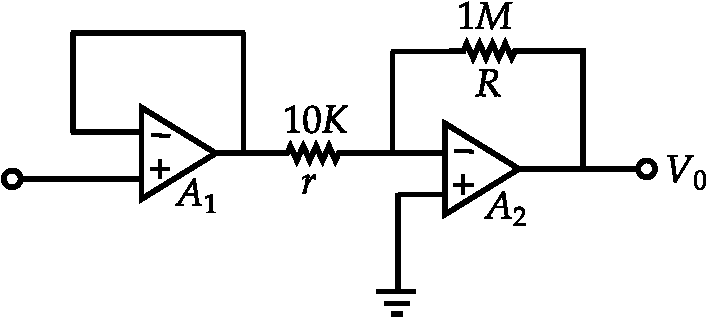
\includegraphics[height=3cm,width=7cm]{e-30}
	\end{figure}
	If the input ac signal source has an impedance of $50 k \Omega$, which of the following statements is true?
{	\exyear{NET/JRF(DEC-2014)}}
\begin{tasks}(1)
\task[\textbf{A.}] $A_{1}$ is required in the circuit because the source impedance is much greater than $r$
\task[\textbf{B.}] $A_{1}$ is required in the circuit because the source impedance is much less than $R$
\task[\textbf{C.}] $A_{1}$ can be eliminated from the circuit without affecting the overall gain
\task[\textbf{D.}] $A_{1}$ is required in the circuit if the output has to follow the phase of the input signal
\end{tasks}
	\item Consider a Low Pass (LP) and a High Pass (HP) filter with cut-off frequencies $f_{L P}$ and $f_{H P}$, respectively, connected in series or in parallel configurations as shown in the Figures A and B below.\\
	\begin{figure}[H]
		\centering
		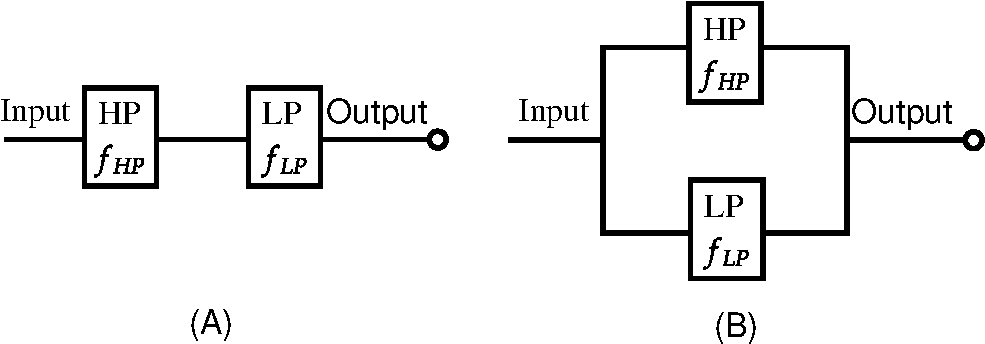
\includegraphics[height=3cm,width=10cm]{e-33}
	\end{figure}
	Which of the following statements is correct?
{	\exyear{NET/JRF(DEC-2014)}}
\begin{tasks}(1)
\task[\textbf{A.}] For $f_{H P}<f_{L P}$, A acts as a Band Pass filter and B acts as a band Reject filter
\task[\textbf{B.}] For $f_{H P}>f_{L P}$, A stops the signal from passing through and B passes the signal without filtering
\task[\textbf{C.}] For $f_{H P}<f_{L P}$, A acts as a Band Pass filter and B passes the signal without filtering
\task[\textbf{D.}] For $f_{H P}>f_{L P}$, A passes the signal without filtering and B acts as a Band Reject filter
\end{tasks}
	\item In the circuit given below, the thermistor has a resistance $3 k \Omega$ at $25^{0} C$. Its resistance decreases by $150 \Omega$ per ${ }^{0} C$ upon heating. The output voltage of the circuit at $30^{\circ} \mathrm{C}$ is
{	\exyear{NET/JRF(JUNE-2015)}}
\begin{figure}[H]
\centering
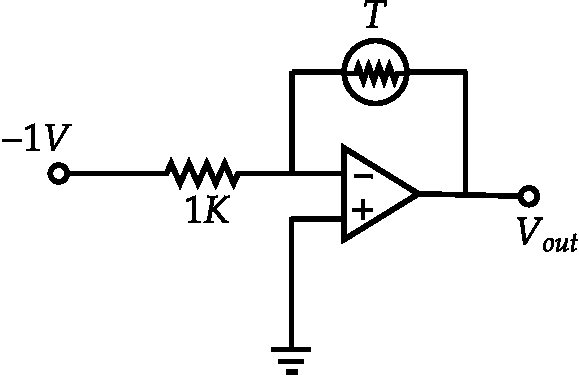
\includegraphics[height=3.3cm,width=5.5cm]{e-38}
\end{figure}
\begin{tasks}(4)
\task[\textbf{A.}] $-3.75 \mathrm{~V}$
\task[\textbf{B.}] $-2.25 \mathrm{~V}$
\task[\textbf{C.}] $2.25 \mathrm{~V}$
\task[\textbf{D.}] $3.75 \mathrm{~V}$
\end{tasks}
	\item If the parameters $y$ and $x$ are related by $y=\log (x)$, then the circuit that can be used to produce an output voltage $V_{0}$ varying linearly with $x$ is
	{\exyear{NET/JRF(DEC-2015)}}
\begin{tasks}(2)
\task[\textbf{A.}] \begin{figure}[H]
	\centering
	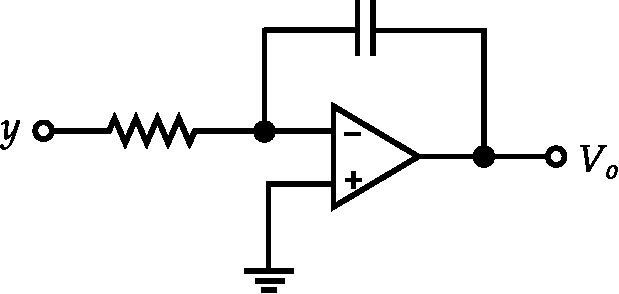
\includegraphics[height=3cm,width=5.5cm]{e40a}
\end{figure}
\task[\textbf{B.}] \begin{figure}[H]
	\centering
	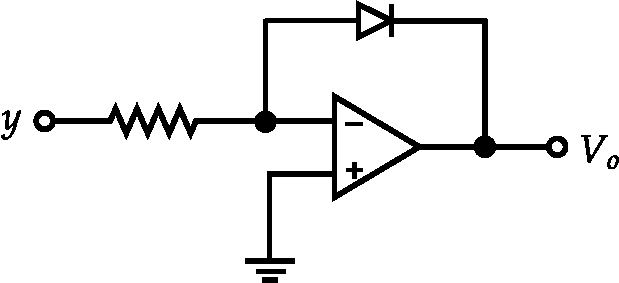
\includegraphics[height=3cm,width=5.5cm]{e40b}
\end{figure}
\task[\textbf{C.}] \begin{figure}[H]
	\centering
	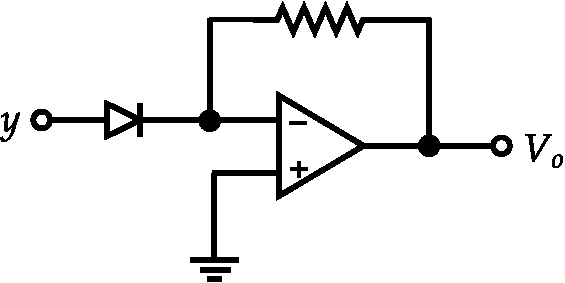
\includegraphics[height=3cm,width=5.5cm]{e40c}
\end{figure}
\task[\textbf{D.}] \begin{figure}[H]
	\centering
	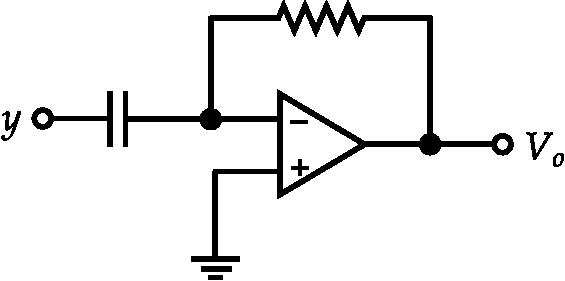
\includegraphics[height=3cm,width=5.5cm]{e40d}
\end{figure}
\end{tasks}
	\item A sinusoidal signal of peak to peak amplitude $1 V$ and unknown time period is input to the following circuit for 5 second's duration. If the counter measures a value $(3 E 8)_{H}$ in hexadecimal, then the time period of the input signal is
{	\exyear{NET/JRF(DEC-2015)}}
\begin{figure}[H]
\centering
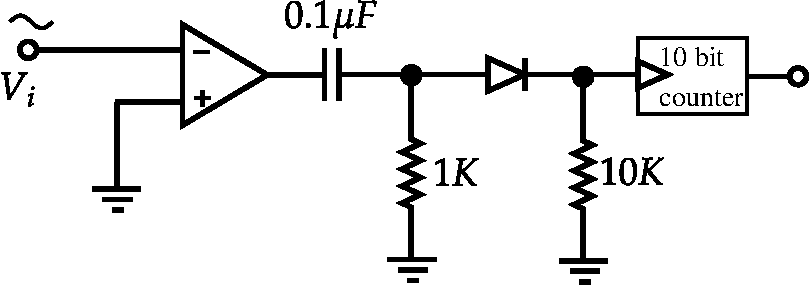
\includegraphics[height=3cm,width=8cm]{e42}
\end{figure}
\begin{tasks}(4)
\task[\textbf{A.}] $2.5 \mathrm{~ms}$
\task[\textbf{B.}] $4 \mathrm{~ms}$
\task[\textbf{C.}]  $10 \mathrm{~ms}$
\task[\textbf{D.}] $5 \mathrm{~ms}$
\end{tasks}
	\item Given the input voltage $V_{i}$, which of the following waveforms correctly represents the output voltage $V_{0}$ in the circuit shown below?
{	\exyear{NET/JRF(JUNE-2016)}}
\begin{figure}[H]
\centering
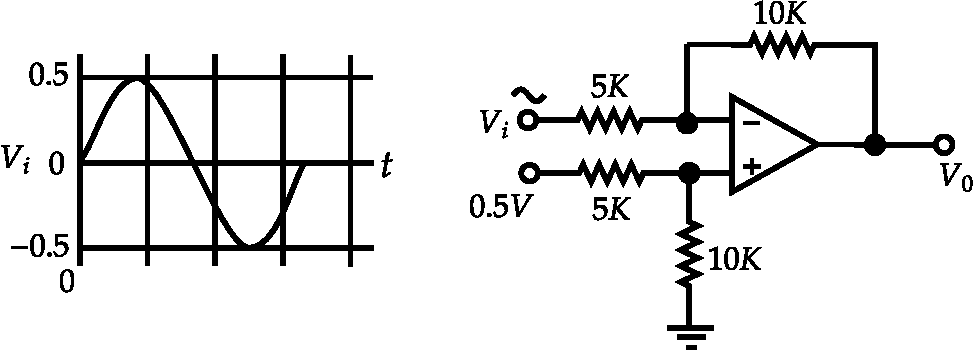
\includegraphics[height=3.5cm,width=10cm]{diagram-20211020(13)-crop}
\end{figure}
\begin{tasks}(2)
\task[\textbf{A.}] \begin{figure}[H]
	\centering
	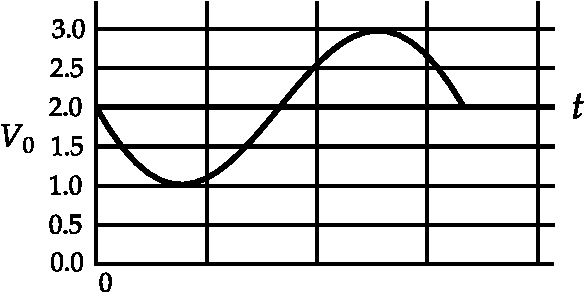
\includegraphics[height=3cm,width=5.5cm]{diagram-20211020(14)-crop}
\end{figure}
\task[\textbf{B.}] \begin{figure}[H]
	\centering
	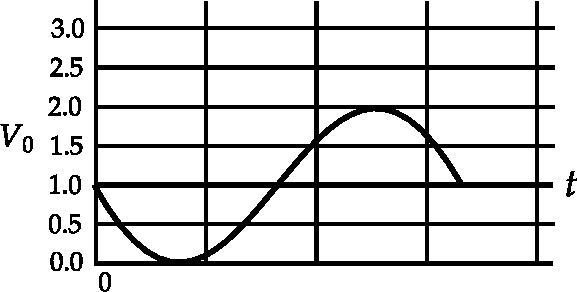
\includegraphics[height=3cm,width=5.5cm]{diagram-20211020(15)-crop}
\end{figure}
\task[\textbf{C.}] \begin{figure}[H]
	\centering
	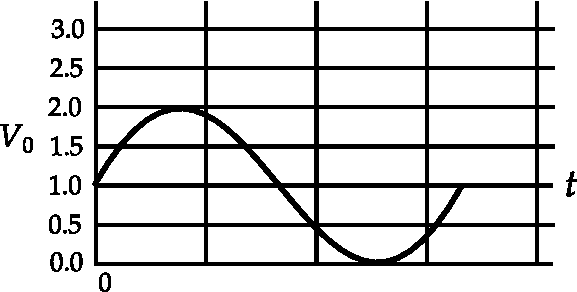
\includegraphics[height=3cm,width=5.5cm]{diagram-20211020(16)-crop}
\end{figure}
\task[\textbf{D.}] \begin{figure}[H]
	\centering
	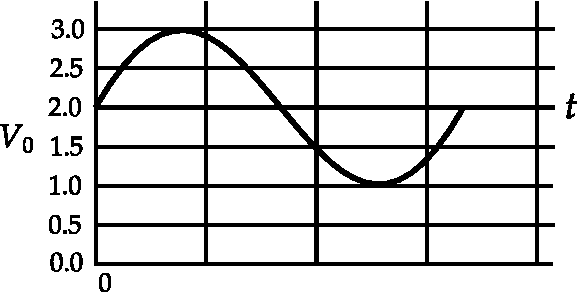
\includegraphics[height=3cm,width=5.5cm]{diagram-20211020(17)-crop}
\end{figure}
\end{tasks}
	\item  In the circuit below, the input voltage $V_{i}$ is $2 V, V_{c c}=16 \mathrm{~V}, R_{2}=2 \mathrm{k} \Omega$ and $R_{L}=10 \mathrm{k} \Omega$\\
	\begin{figure}[H]
		\centering
		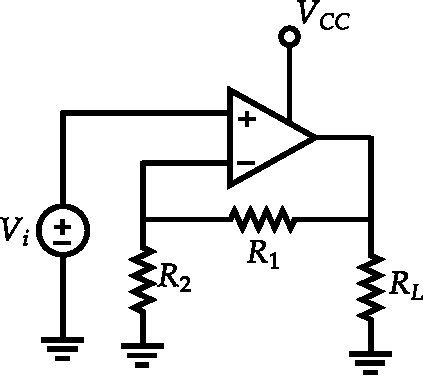
\includegraphics[height=3.5cm,width=4.5cm]{e50}
	\end{figure}
	The value of $R_{1}$ required to deliver $10 \mathrm{~mW}$ of power across $R_{L}$ is
	{\exyear{NET/JRF(DEC-2016)}}
\begin{tasks}(4)
\task[\textbf{A.}] $12 k \Omega$
\task[\textbf{B.}] $4 k \Omega$
\task[\textbf{C.}]  $8 \mathrm{k} \Omega$
\task[\textbf{D.}]  $14 k \Omega$
\end{tasks}                
	\item The gain of the circuit given below is $-\frac{1}{\omega R C}$.\\
	\begin{figure}[H]
		\centering
		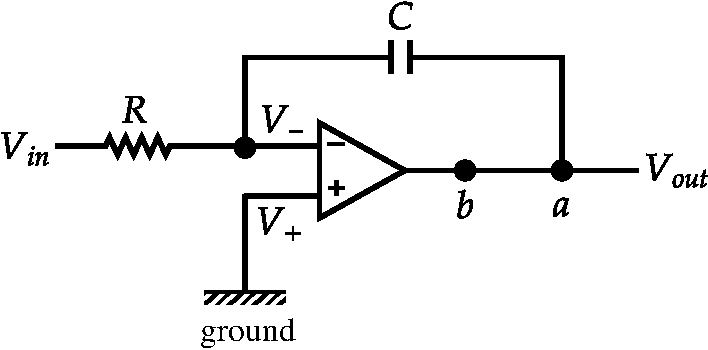
\includegraphics[height=3.5cm,width=6.5cm]{e54}
	\end{figure}
	The modification in the circuit required to introduce a dc feedback is to add a resistor
	{\exyear{NET/JRF(JUNE-2017)}}
\begin{tasks}(1)
\task[\textbf{A.}] Between $a$ and $b$
\task[\textbf{B.}]  Between positive terminal of the op-amp and ground
\task[\textbf{C.}] In series with $C$
\task[\textbf{D.}] Parallel to $C$
\end{tasks}
	\item In the following operational amplifier circuit $C_{i n}=10 n F, R_{i n}=20 k \Omega, R_{F}=200 k \Omega$ and $C_{F}=100 \mathrm{pF}$\\
	\begin{figure}[H]
		\centering
		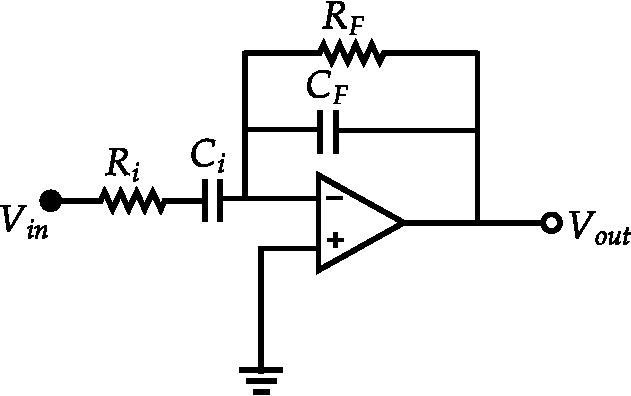
\includegraphics[height=3.5cm,width=6cm]{e60}
	\end{figure}
	The magnitude of the gain at a input signal frequency of $16 \mathrm{kHz}$ is
	{\exyear{NET/JRF(JUNE-2017)}}
\begin{tasks}(4)
\task[\textbf{A.}] 67
\task[\textbf{B.}] $0.15$
\task[\textbf{C.}] $0.3$
\task[\textbf{D.}] $3.5$
\end{tasks}
	\item Two signals $A_{1} \sin (\omega t)$ and $A_{2} \cos (\omega t)$ are fed into the input and the reference channels, respectively, of a lock-in amplifier. The amplitude of each signal is $1 V$. The time constant of the lock-in amplifier is such that any signal of frequency larger than $\omega$ is filtered out. The output of the lock-in amplifier is
	{\exyear{NET/JRF(JUNE-2018)}}
\begin{tasks}(4)
\task[\textbf{A.}]  $2 V$
\task[\textbf{B.}] $1 \mathrm{~V}$
\task[\textbf{C.}] $0.5 \mathrm{~V}$
\task[\textbf{D.}] $0 V$
\end{tasks}
	\item The input $V_i$ to the following circuit is a square wave as shown in the following figure\\
	\begin{figure}[H]
		\centering
		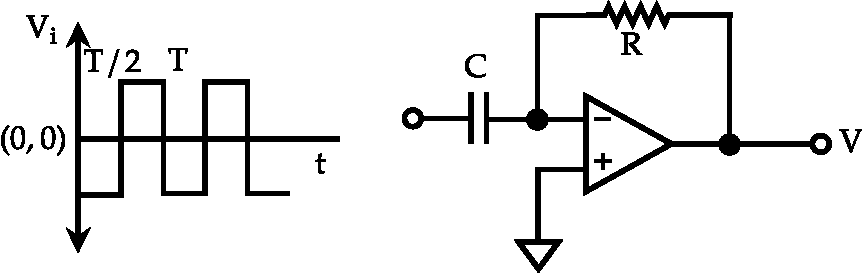
\includegraphics[height=3cm,width=8cm]{e73}
	\end{figure}
	Which of the waveforms $V_0$ best describes the output?
{	\exyear{NET/JRF(JUNE-2018)}}
\begin{tasks}(2)
\task[\textbf{A.}] \begin{figure}[H]
	\centering
	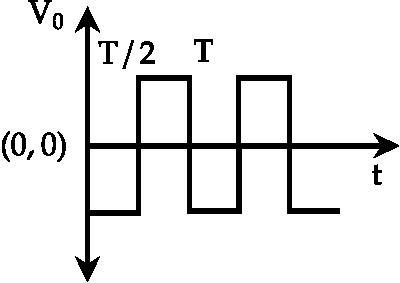
\includegraphics[height=3cm,width=5cm]{e73a}
\end{figure}
\task[\textbf{B.}] \begin{figure}[H]
	\centering
	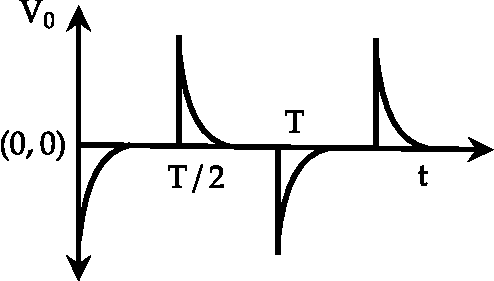
\includegraphics[height=3cm,width=5cm]{e73b}
\end{figure}
\task[\textbf{C.}] \begin{figure}[H]
	\centering
	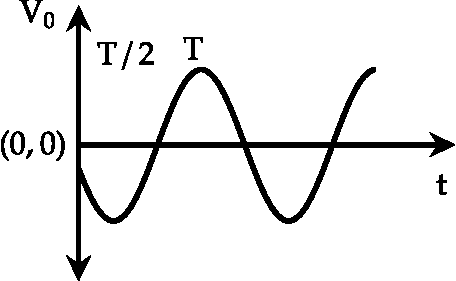
\includegraphics[height=3cm,width=5cm]{e73c}
\end{figure}
\task[\textbf{D.}] \begin{figure}[H]
	\centering
	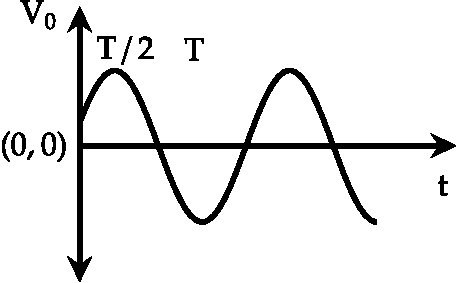
\includegraphics[height=3cm,width=5cm]{e73d}
\end{figure}
\end{tasks}
	\item The input $V_ i$ to the following circuit is a square wave as shown in the following figure.\\
	\begin{figure}[H]
		\centering
		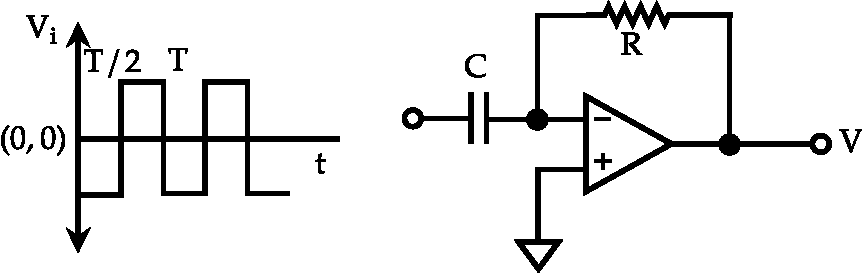
\includegraphics[height=2.5cm,width=8cm]{e73}
	\end{figure}
	which of the waveforms best describes the output?
{	\exyear{NET/JRF(DEC-2018)}}
\begin{tasks}(2)
\task[\textbf{A.}] \begin{figure}[H]
	\centering
	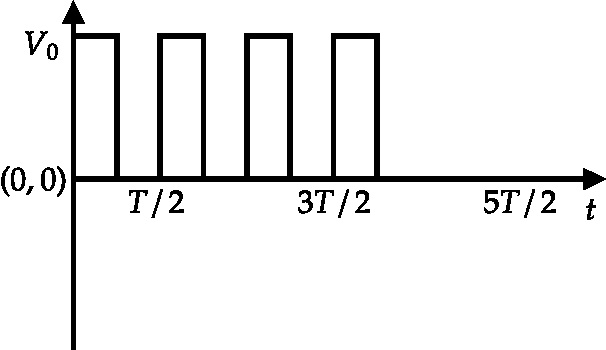
\includegraphics[height=3cm,width=5cm]{e74a}
\end{figure}
\task[\textbf{B.}] \begin{figure}[H]
	\centering
	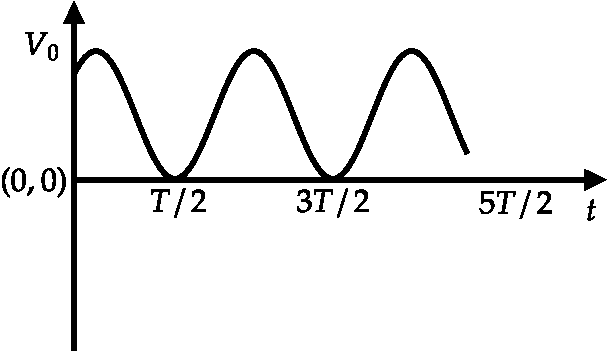
\includegraphics[height=3cm,width=5cm]{e74b}
\end{figure}
\task[\textbf{C.}] \begin{figure}[H]
	\centering
	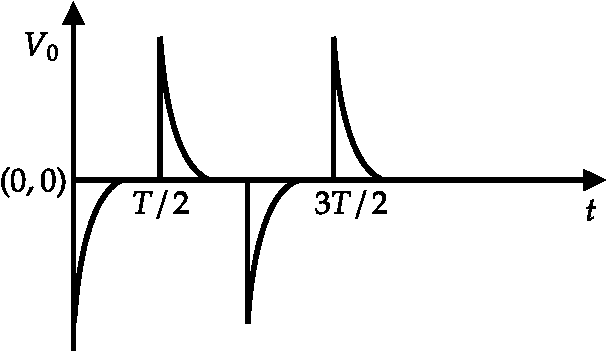
\includegraphics[height=3cm,width=5cm]{e74c}
\end{figure}
\task[\textbf{D.}]\begin{figure}[H]
	\centering
	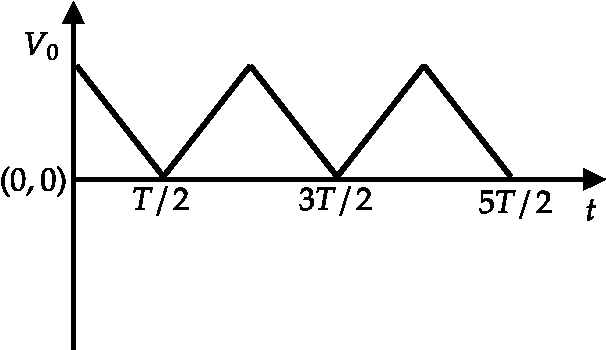
\includegraphics[height=3cm,width=5cm]{e74d}
\end{figure}
\end{tasks}
	\item A circuit constructed using op-amp, resistor $R_{1}=1 \mathrm{k} \Omega$ and capacitors $C_{1}=1 \mu \mathrm{F}$ and $C_{2}=0.1 \mu F$ is shown in the figure below.\\
	\begin{figure}[H]
		\centering
		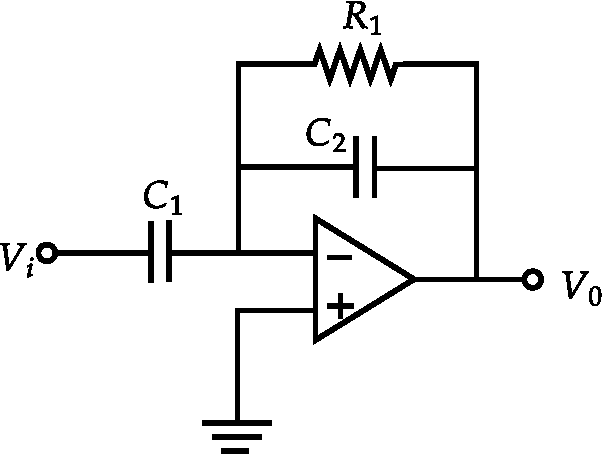
\includegraphics[height=4cm,width=5cm]{diagram-20211029(7)-crop}
	\end{figure}
	This circuit will act as a
{	\exyear{NET/JRF(JUNE-2019)}}
\begin{tasks}(2)
\task[\textbf{A.}] High pass filter
\task[\textbf{B.}] Low pass filter
\task[\textbf{C.}] Band pass filter
\task[\textbf{D.}] Band reject filter
\end{tasks}
	\item In the circuit diagram of a band pass filter shown below, $R=10 \mathrm{k} \Omega$.\\
	\begin{figure}[H]
		\centering
		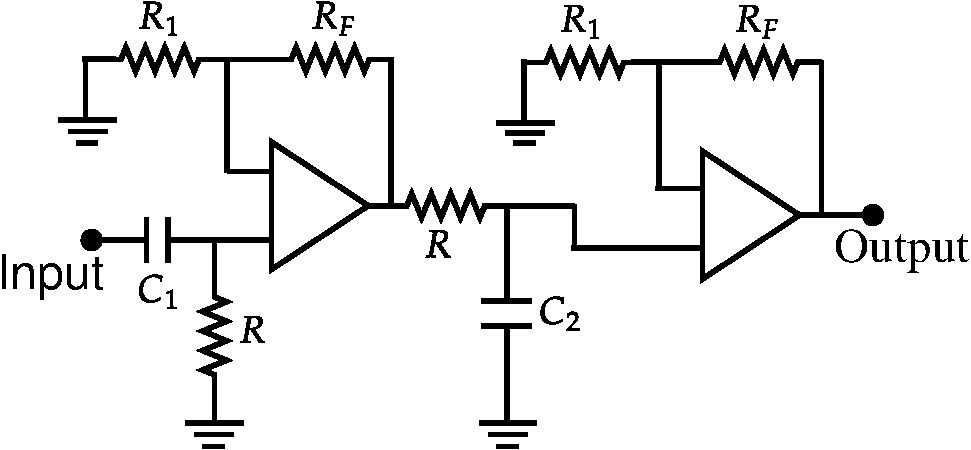
\includegraphics[height=3.5cm,width=8cm]{diagram-20211029(10)-crop}
	\end{figure}
	In order to get a lower cut-off frequency of $150 \mathrm{~Hz}$ and an upper cut-off frequency of $10 \mathrm{kHz}$, the appropriate values of $C_{1}$ and $C_{2}$ respectively are
{	\exyear{NET/JRF(DEC-2019)}}
\begin{tasks}(2)
\task[\textbf{A.}]  $0.1 \mu F$ and $1.5 n F$
\task[\textbf{B.}] $0.3 \mu \mathrm{F}$ and $5.0 \mathrm{nF}$
\task[\textbf{C.}] $1.5 n F$ and $0.1 \mu F$
\task[\textbf{D.}]  $5.0 \mathrm{nF}$ and $0.3 \mu \mathrm{F}$
\end{tasks}
	\item The $I-V$ characteristics of the diode $D$ in the circuit below is given by
	$$
	I=I_{s}\left(e^{\frac{q V}{k_{\mathrm{B}} T}}-1\right)
	$$
	where $I_{s}$ is the reverse saturation current, $V$ is the voltage across the diode and $T$ is the absolute temperature.\\
	\begin{figure}[H]
		\centering
		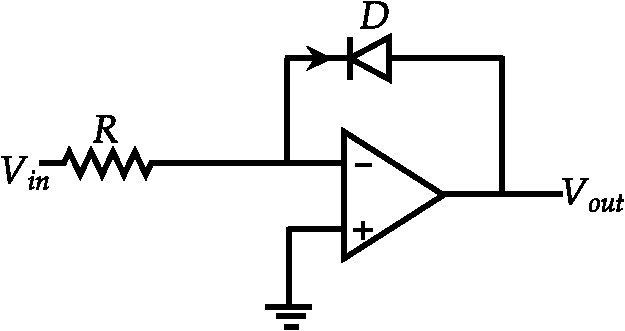
\includegraphics[height=3.5cm,width=6cm]{diagram-20211030(4)-crop}
		\caption{}
		\label{}
	\end{figure}
	If the input voltage is $V_{\text {in }}$, then the output voltage $V_{\text {out }}$ is
{	\exyear{NET/JRF(JUNE-2020)}}
\begin{tasks}(2)
\task[\textbf{A.}] (a) $I_{s} R \ln \left(\frac{q V_{\text {in }}}{k_{B} T}+1\right)$
\task[\textbf{B.}] $\frac{1}{q} k_{B} T \ln \left(\frac{q\left(V_{\text {in }}+I_{s} R\right)}{k_{B} T}\right)$
\task[\textbf{C.}]  $\frac{1}{q} k_{B} T \ln \left(\frac{V_{\text {in }}}{I_{s} R}+1\right)$
\task[\textbf{D.}]  $-\frac{1}{q} k_{B} T \ln \left(\frac{V_{\text {in }}}{I_{s} R}+1\right)$
\end{tasks}
	\item In the circuit shown below, the gain of the op-amp in the middle of its bandwidth is $10^{5}$. A sinusoidal voltage with angular frequency $\omega=100 \mathrm{rad} / \mathrm{s}$ is applied to the input of the op-amp.\\
	\begin{figure}[H]
		\centering
		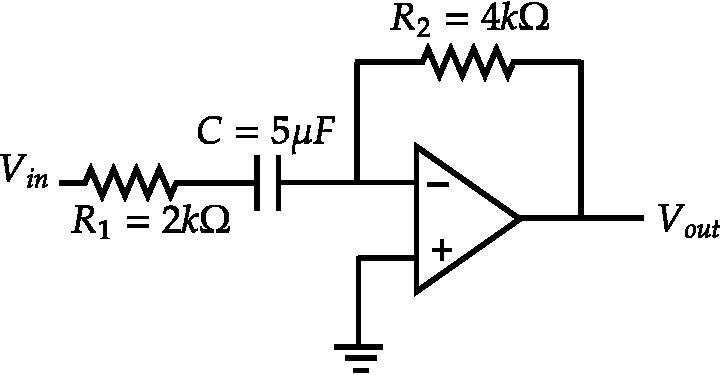
\includegraphics[height=4cm,width=7cm]{diagram-20211030(5)-crop}
		\caption{}
		\label{}
	\end{figure}
	The phase difference between the input and the output voltage is
{	\exyear{NET/JRF(JUNE-2020)}}
\begin{tasks}(4)
\task[\textbf{A.}]  $5 \pi / 4$
\task[\textbf{B.}] $3 \pi / 4$
\task[\textbf{C.}] $\pi / 2$
\task[\textbf{D.}] $\pi$
\end{tasks}
\end{enumerate}
 \colorlet{ocre1}{ocre!70!}
\colorlet{ocrel}{ocre!30!}
\setlength\arrayrulewidth{1pt}
\begin{table}[H]
	\centering
	\arrayrulecolor{ocre}
	\begin{tabular}{|p{1.5cm}|p{1.5cm}||p{1.5cm}|p{1.5cm}|}
		\hline
		\multicolumn{4}{|c|}{\textbf{Answer key}}\\\hline\hline
		\rowcolor{ocrel}Q.No.&Answer&Q.No.&Answer\\\hline
		1&\textbf{C} &2&\textbf{B}\\\hline 
		3&\textbf{B} &4&\textbf{D} \\\hline
		5&\textbf{C} &6&\textbf{A} \\\hline
		7&\textbf{A}&8&\textbf{C}\\\hline
		9&\textbf{C}&10&\textbf{C}\\\hline
		11&\textbf{D} &12&\textbf{B}\\\hline
		13&\textbf{C}&14&\textbf{D}\\\hline
		15&\textbf{D}&16&\textbf{D} \\\hline
		17&\textbf{B}&18&\textbf{C}\\\hline
		19&\textbf{A}&20&\textbf{A}\\\hline
		21&\textbf{C} &22&\textbf{A}\\\hline
		
	\end{tabular}
\end{table}
 \newpage
 \begin{abox}
 	Practice Set- 2
 \end{abox}
 \begin{enumerate}
 	\item In one of the following circuits, negative feedback does not operate for a negative input. Which one is it? The opamps are running from $\pm 15 \mathrm{~V}$ supplies.
 	{\exyear{GATE 2010}}
 	\begin{tasks}(2)
 		\task[\textbf{A.}] \begin{figure}[H]
 			\centering
 			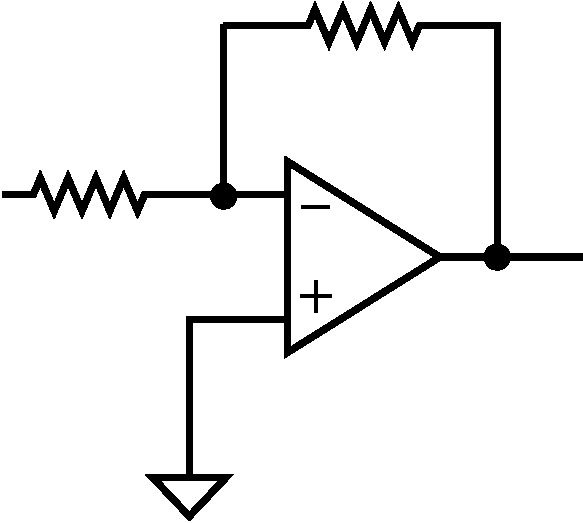
\includegraphics[height=3.5cm,width=4cm]{diagram-20210912(9)-crop}
 		\end{figure}
 		\task[\textbf{B.}] \begin{figure}[H]
 			\centering
 			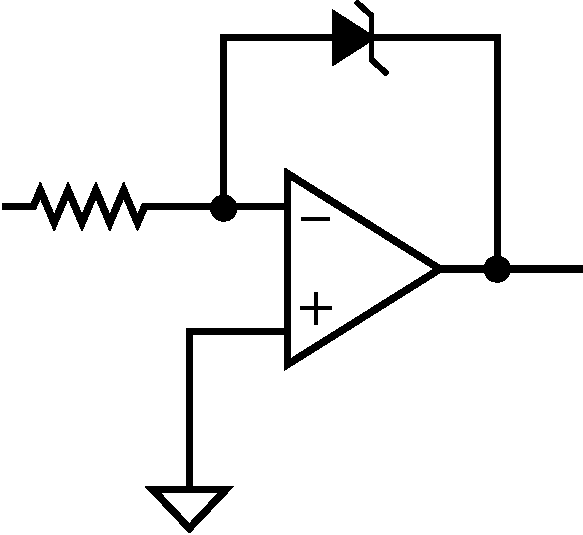
\includegraphics[height=3.5cm,width=4cm]{diagram-20210912(10)-crop}
 		\end{figure}
 		\task[\textbf{C.}] \begin{figure}[H]
 			\centering
 			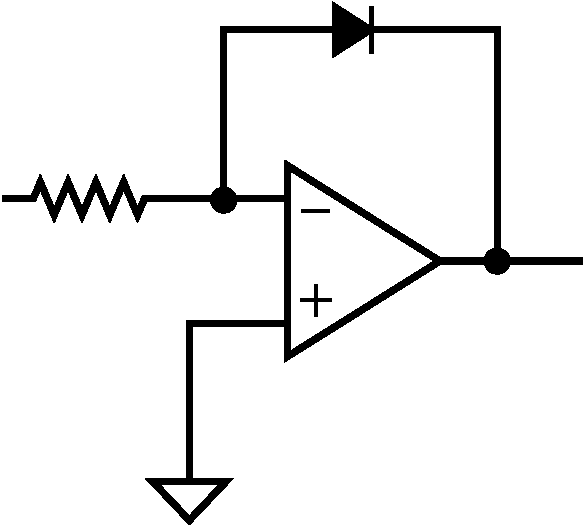
\includegraphics[height=3.5cm,width=4cm]{diagram-20210912(11)-crop}
 		\end{figure}
 		\task[\textbf{D.}] \begin{figure}[H]
 			\centering
 			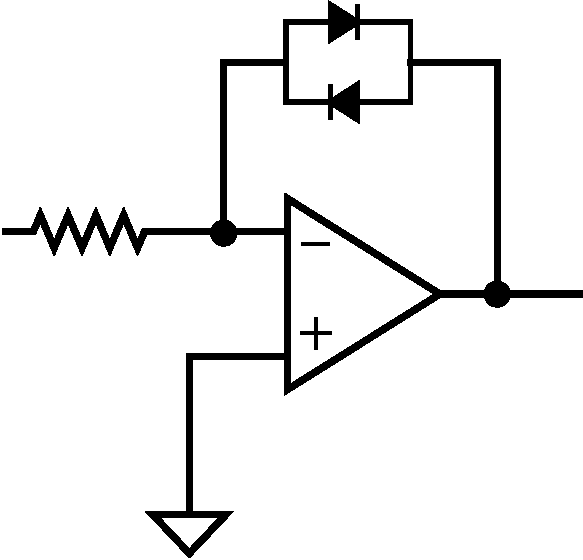
\includegraphics[height=3.5cm,width=4cm]{diagram-20210912(12)-crop}
 		\end{figure}
 	\end{tasks}
 	\item Consider the following circuit.\\
 	\begin{figure}[H]
 		\centering
 		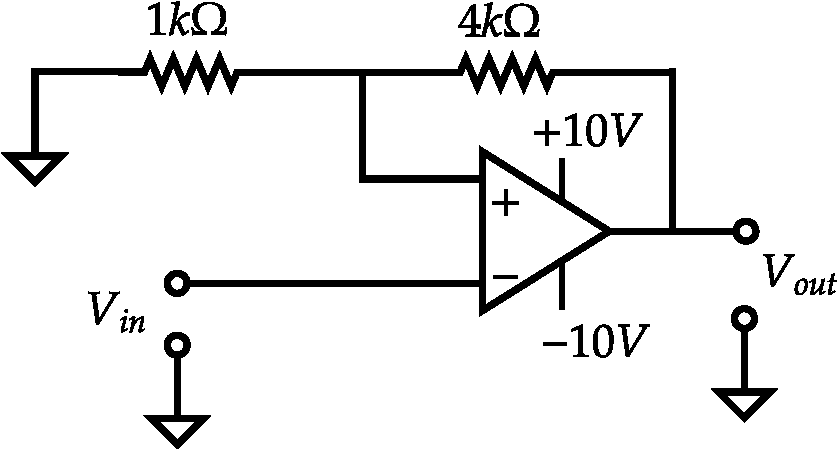
\includegraphics[height=4cm,width=7.5cm]{diagram-20210913(6)-crop}
 	\end{figure}
 	Which of the following correctly represents the output $V_{\text {out }}$ corresponding to the input $V_{i n} ?$
 	{\exyear{GATE 2011}}
 	\begin{tasks}(2)
 		\task[\textbf{A.}] \begin{figure}[H]
 			\centering
 			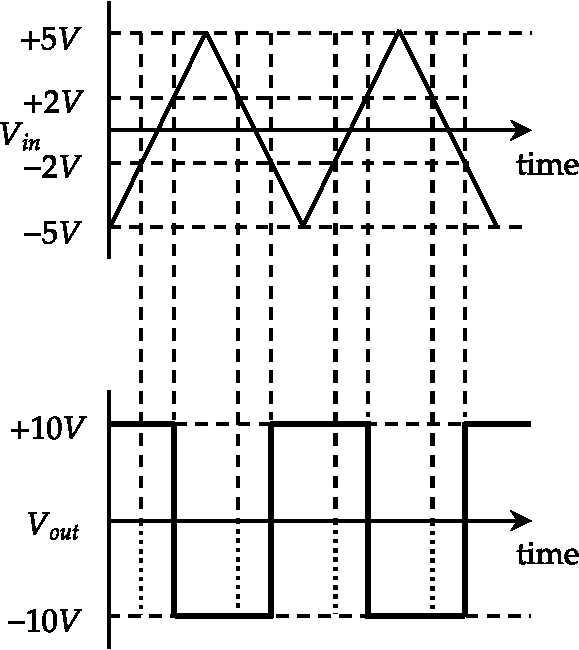
\includegraphics[height=6.5cm,width=6cm]{diagram-20210913(2)-crop}
 		\end{figure}
 		\task[\textbf{B.}] \begin{figure}[H]
 			\centering
 			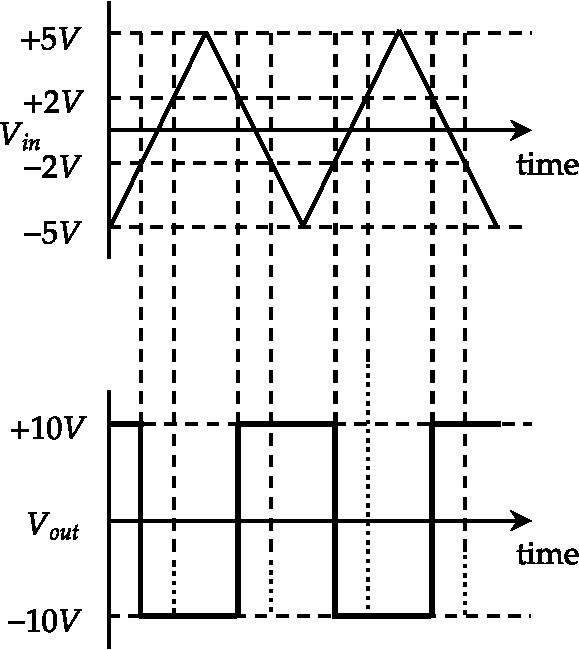
\includegraphics[height=6.5cm,width=6cm]{diagram-20210913(3)-crop}
 		\end{figure}
 		\task[\textbf{C.}]\begin{figure}[H]
 			\centering
 			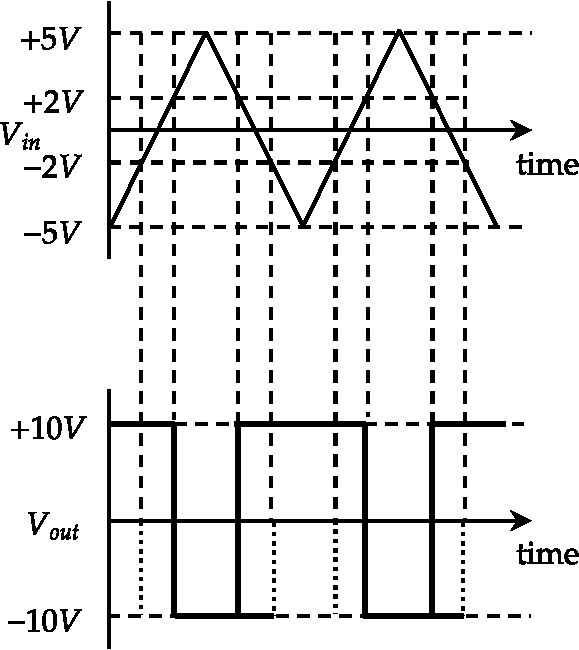
\includegraphics[height=6.5cm,width=6cm]{diagram-20210913(4)-crop}
 		\end{figure}
 		\task[\textbf{D.}] \begin{figure}[H]
 			\centering
 			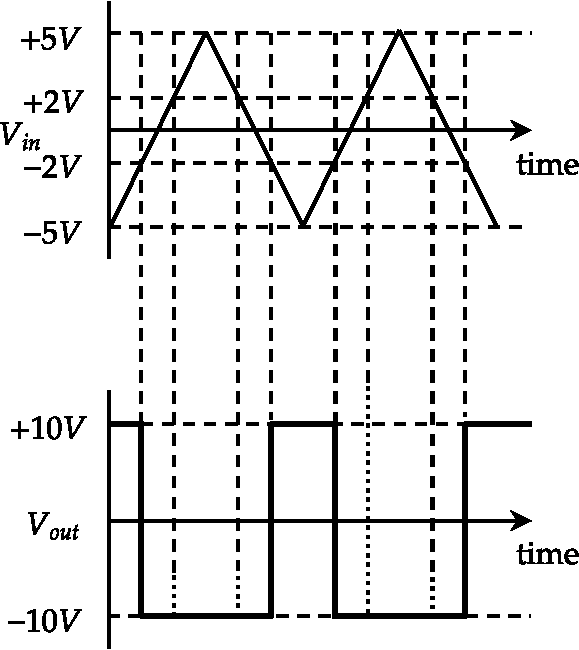
\includegraphics[height=6.5cm,width=6cm]{diagram-20210913(5)-crop}
 		\end{figure}
 	\end{tasks}
 	\item If the peak output voltage of a full wave rectifier is $10 \mathrm{~V}$, its d.c. voltage is
 	{	\exyear{GATE 2012}}
 	\begin{tasks}(4)
 		\task[\textbf{A.}] $10.0 \mathrm{~V}$
 		\task[\textbf{B.}] $7.07 \mathrm{~V}$
 		\task[\textbf{C.}] $6.36 \mathrm{~V}$
 		\task[\textbf{D.}] $3.18 \mathrm{~V}$
 	\end{tasks}
 	\item In the following circuit, for the output voltage to be $V_{0}=\left(-V_{1}+V_{2} / 2\right)$ the ratio $R_{1} / R_{2}$ is
 	{	\exyear{GATE 2012}}
 	\begin{figure}[H]
 		\centering
 		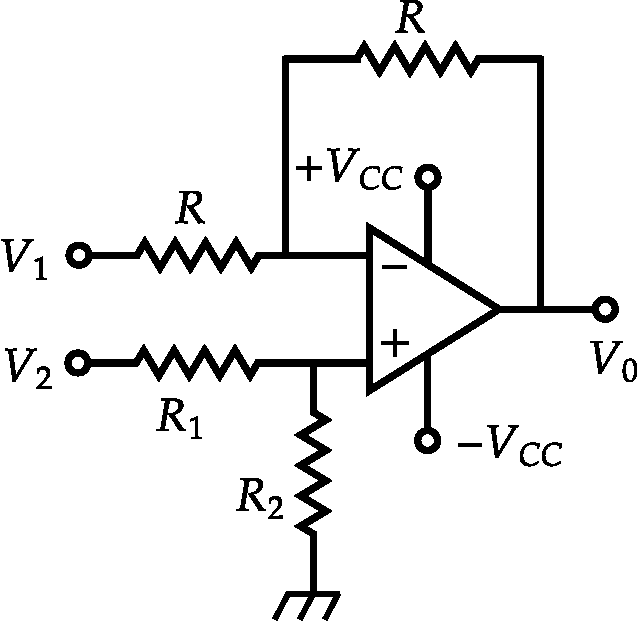
\includegraphics[height=6.5cm,width=6.5cm]{diagram-20210913(12)-crop}
 	\end{figure}
 	\begin{tasks}(4)
 		\task[\textbf{A.}] $1 / 2$
 		\task[\textbf{B.}] 1
 		\task[\textbf{C.}] 2
 		\task[\textbf{D.}] 3
 	\end{tasks}
 	\item Consider the following OP-AMP circuit.
 	Which one of the following correctly represents the output $\mathrm{V}_{\text {out }}$ corresponding to the input $\mathrm{V}_{\text {in }}$ ?
 	{	\exyear{GATE 2012}}
 	\begin{figure}[H]
 		\centering
 		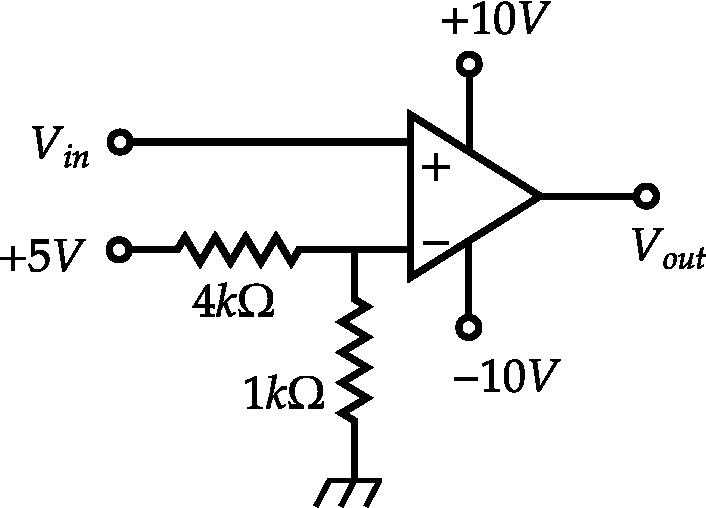
\includegraphics[height=5.5cm,width=7cm]{diagram-20210913(13)-crop}
 	\end{figure}
 	\begin{tasks}(2)
 		\task[\textbf{A.}] \begin{figure}[H]
 			\centering
 			\includegraphics[height=6cm,width=5cm]{diagram-20210913(15)-crop}
 		\end{figure}
 		\task[\textbf{B.}] \begin{figure}[H]
 			\centering
 			\includegraphics[height=6cm,width=5cm]{diagram-20210913(16)-crop}
 		\end{figure}
 		\task[\textbf{C.}] \begin{figure}[H]
 			\centering
 			\includegraphics[height=6cm,width=5cm]{diagram-20210913(17)-crop}
 		\end{figure}
 		\task[\textbf{D.}] \begin{figure}[H]
 			\centering
 			\includegraphics[height=6cm,width=5cm]{diagram-20210913(18)-crop}
 		\end{figure}
 	\end{tasks}
 	\item For this circuit the frequency above which the gain will decrease by $20 d B$ per decade is
 	{	\exyear{GATE 2013}}
 	\begin{figure}[H]
 		\centering
 		\includegraphics[height=5cm,width=9cm]{diagram-20210913(28)-crop}
 	\end{figure}
 	\begin{tasks}(4)
 		\task[\textbf{A.}] $15.9 \mathrm{kHz}$
 		\task[\textbf{B.}] $1.2 \mathrm{kHz}$
 		\task[\textbf{C.}]  $5.6 \mathrm{kHz}$
 		\task[\textbf{D.}] $22.5 \mathrm{kHz}$
 	\end{tasks}
 	\item At $1.2 \mathrm{kHz}$ the closed loop gain is
 	{\exyear{GATE 2013}}
 	\begin{tasks}(4)
 		\task[\textbf{A.}] 1
 		\task[\textbf{B.}] $1.5$
 		\task[\textbf{C.}]  3
 		\task[\textbf{D.}]  $0.5$
 	\end{tasks}
 	\item The input given to an ideal OP-AMP integrator circuit is\\
 	\begin{figure}[H]
 		\centering
 		\includegraphics[height=3cm,width=6cm]{diagram-20210913(29)-crop}
 	\end{figure}
 	The correct output of the integrator circuit is
 	{	\exyear{GATE 2014}}
 	\begin{tasks}(2)
 		\task[\textbf{A.}] \begin{figure}[H]
 			\centering
 			\includegraphics[height=3cm,width=6cm]{diagram-20210913(30)-crop}
 		\end{figure}
 		\task[\textbf{B.}] \begin{figure}[H]
 			\centering
 			\includegraphics[height=3cm,width=6cm]{diagram-20210913(31)-crop}
 		\end{figure}
 		\task[\textbf{C.}] \begin{figure}[H]
 			\centering
 			\includegraphics[height=3cm,width=6cm]{diagram-20210913(32)-crop}
 		\end{figure}
 		\task[\textbf{D.}] \begin{figure}[H]
 			\centering
 			\includegraphics[height=3cm,width=6cm]{diagram-20210913(33)-crop}
 		\end{figure}
 	\end{tasks}
 	\item A low pass filter is formed by a resistance $R$ and a capacitance $C .$ At the cut-off angular frequency $\omega_{C}=\frac{1}{R C}$ the voltage gain and the phase of the output voltage relative to the input voltage respectively are
 	{	\exyear{GATE 2014}}
 	\begin{tasks}(4)
 		\task[\textbf{A.}] $0.71$ and $45^{\circ}$
 		\task[\textbf{B.}]  $0.71$ and $-45^{\circ}$
 		\task[\textbf{C.}] $0.5$ and $-90^{\circ}$
 		\task[\textbf{D.}] $0.5$ and $90^{\circ}$
 	\end{tasks}
 	\item Consider the circuit shown in the figure, where $R C=1$. For an input signal $V_{i}$ shown below, choose the correct $V_{0}$ from the options:
 	{	\exyear{GATE 2015}}
 	\begin{figure}[H]
 		\centering
 		\includegraphics[height=4.5cm,width=12cm]{diagram-20210913(42)-crop}
 	\end{figure}
 	\begin{tasks}(2)
 		\task[\textbf{A.}] \begin{figure}[H]
 			\centering
 			\includegraphics[height=4.5cm,width=6.5cm]{diagram-20210913(37)-crop}
 		\end{figure}
 		\task[\textbf{B.}] \begin{figure}[H]
 			\centering
 			\includegraphics[height=4.5cm,width=6.5cm]{diagram-20210913(38)-crop}
 		\end{figure}
 		\task[\textbf{C.}] \begin{figure}[H]
 			\centering
 			\includegraphics[height=4.5cm,width=6.5cm]{diagram-20210913(39)-crop}
 		\end{figure}
 		\task[\textbf{D.}]\begin{figure}[H]
 			\centering
 			\includegraphics[height=4.5cm,width=6.5cm]{diagram-20210913(40)-crop}
 		\end{figure}
 	\end{tasks}
 	\item In the given circuit, if the open loop gain $A=10^{5}$ the feedback configurations and the closed loop gain $A_{f}$ are
 	{	\exyear{GATE 2015}}
 	\begin{figure}[H]
 		\centering
 		\includegraphics[height=4cm,width=6cm]{diagram-20210914(2)-crop}
 	\end{figure}
 	\begin{tasks}(2)
 		\task[\textbf{A.}] series-shunt, $A_{f}=9$
 		\task[\textbf{B.}] series-series, $A_{f}=10$
 		\task[\textbf{C.}] series-shunt, $A_{f}=10$
 		\task[\textbf{D.}] shunt-shunt, $A_{f}=10$
 	\end{tasks}
 	\item Consider an ideal operational amplifier as shown in the figure below with $R_{1}=5 k \Omega, R_{2}=1 k \Omega, R_{L}=100 k \Omega .$ For an applied input voltage $V=10 \mathrm{mV}$, the current passing through $R_{2}$ is............... $\mu A$. (up to two decimal places)
 	{\exyear{GATE 2017}}
 	\begin{figure}[H]
 		\centering
 		\includegraphics[height=4cm,width=6.5cm]{diagram-20210914(12)-crop}
 	\end{figure}
 	\item For an operational amplifier (ideal) circuit shown below,\\
 	\begin{figure}[H]
 		\centering
 		\includegraphics[height=4cm,width=7cm]{diagram-20210914(30)-crop}
 		\caption{}
 		\label{}
 	\end{figure}
 	If $V_{1}=1 V$ and $V_{2}=2 V$, the value of $V_{0}$ is ---------$V$ (up to one decimal place).
 	{	\exyear{GATE 2018}}
 	\item For the following circuit, what is the magnitude of $V_{\text {out }}$ if $V_{\text {in }}=1.5 V$ ?
 	{	\exyear{IIT JAM 2018}}
 	\begin{figure}[H]
 		\centering
 		\includegraphics[height=5cm,width=7cm]{diagram-20210914(21)-crop}
 	\end{figure}
 	\begin{tasks}(4)
 		\task[\textbf{A.}] $0.015 \mathrm{~V}$
 		\task[\textbf{B.}] $0.15 \mathrm{~V}$
 		\task[\textbf{C.}] $15 \mathrm{~V}$
 		\task[\textbf{D.}] $150 \mathrm{~V}$
 	\end{tasks}
 	\item What is the voltage at the output of the following operational amplifier circuit. [See in the figure]?
 	{	\exyear{JEST 2015}}
 	\begin{figure}[H]
 		\centering
 		\includegraphics[height=5.5cm,width=7cm]{diagram-20210816(10)-crop}
 	\end{figure}
 	\begin{tasks}(4)
 		\task[\textbf{A.}] $1 \mathrm{~V}$
 		\task[\textbf{B.}] $1 \mathrm{mV}$
 		\task[\textbf{C.}] $1 \mu V$
 		\task[\textbf{D.}] $1 n V$
 	\end{tasks}
 	\item Consider a 741 operational amplifier circuit as shown below, where $V_{C C}=V_{E E}=+15 V$ and $R=2.2 \mathrm{k} \Omega$. If $v_{I}=2 m V$, what is the value of $v_{0}$ with respect to the ground?
 	{	\exyear{JEST 2017}}
 	\begin{figure}[H]
 		\centering
 		\includegraphics[height=5.5cm,width=7cm]{diagram-20210816(29)-crop}
 	\end{figure}
 	\begin{tasks}(4)
 		\task[\textbf{A.}] $-1 \mathrm{mV}$
 		\task[\textbf{B.}] $-2 m V$
 		\task[\textbf{C.}] $-3 m V$
 		\task[\textbf{D.}] $-4 m V$
 	\end{tasks}
 	\item Analyse the ideal op-amp circuit in the figure. Which one of the following statements is true about the output voltage $V_{\text {out }}$, when terminal ' $C$ ' is connected to point ' $A$ ' and then to point ' $B$ '?
 	{\exyear{JEST 2019}}
 	\begin{figure}[H]
 		\centering
 		\includegraphics[height=4.5cm,width=6cm]{diagram-20210817(1)-crop}
 	\end{figure}
 	\begin{tasks}(1)
 		\task[\textbf{A.}] $V_{\text {out }}=V_{\text {in }}$ and $V_{\text {out }}=-V_{\text {in }}$ when ' $C$ ' is connected to ' $A$ ' and ' $B$ ', respectively
 		\task[\textbf{B.}] $V_{\text {out }}=-V_{\text {in }}$ and $V_{\text {out }}=V_{\text {in }}$ when ' $C$ ' is connected to ' $A$ ' and ' $B$ ', respectively
 		\task[\textbf{C.}] $V_{\text {out }}=-V_{\text {in }}$ when ' $C$ ' is connected to either ' $A$ ' or ' $B$ '
 		\task[\textbf{D.}]  $V_{\text {out }}=V_{\text {in }}$ when ' $C$ ' is connected to either ' $A$ ' or ' $B$ '
 	\end{tasks}

 \end{enumerate}
 \colorlet{ocre1}{ocre!70!}
\colorlet{ocrel}{ocre!30!}
\setlength\arrayrulewidth{1pt}
\begin{table}[H]
	\centering
	\arrayrulecolor{ocre}
	\begin{tabular}{|p{1.5cm}|p{1.5cm}||p{1.5cm}|p{1.5cm}|}
		\hline
		\multicolumn{4}{|c|}{\textbf{Answer key}}\\\hline\hline
		\rowcolor{ocrel}Q.No.&Answer&Q.No.&Answer\\\hline
		1&\textbf{C} &2&\textbf{A}\\\hline 
		3&\textbf{C} &4&\textbf{D} \\\hline
		5&\textbf{A} &6&\textbf{A} \\\hline
		7&\textbf{B}&8&\textbf{A}\\\hline
		9&\textbf{B}&10&\textbf{B}\\\hline
		11&\textbf{C} &12&\textbf{10$\mu A$}\\\hline
		13&\textbf{-3.6V}&14&\textbf{C}\\\hline
		15&\textbf{B}&16&\textbf{C}\\\hline
		17&\textbf{A}&&\textbf{}\\\hline
	\end{tabular}
\end{table}